% ============================================================
% PART II OF THE SCIENTIFIC PROPOSAL (max. 7 pages)
% References do not count towards the page limit.
% ============================================================
% Header: Lepperød — FIND — Part B2

\section{Part II of the Scientific Proposal}

This section details the research methodology, work plan, and risk assessment for FIND. Part II complements Part I by providing the implementation specifics; it should not be read as a repetition of Part I but as a detailed elaboration of how the objectives will be achieved.

\textbf{Research questions:}
\begin{itemize}[noitemsep,topsep=2pt]
  \item Q1: How can memory-augmented modules distribute and combine long-term temporal information?
  \item Q2: How can such modules support active inference and causal reasoning?
  \item Q3: How can neurosymbolic components be integrated into distributed memory architectures without sacrificing gradient-based learning?
  \item Q4: Does this integration measurably enhance compositional reasoning in complex environments?
  \item Q5: Can such networks learn adaptively and reason about causal relations over long time horizons?
\end{itemize}

\subsection{Research methodology}

The core update equations underpin PAM's mechanisms. Each module $m$ has latent state $z^m_t \in \mathbb{R}^{d_z}$ and sensory input $x^m_t \in \mathbb{R}^{d_x}$ at time $t$. The prediction error $e_t = x^m_t - \hat{x}^m_t$ drives module state updates: $z^m_{t+1} = f_m(z^m_t, c^m_t, r^m_t, a_t)$, where $f_m$ is a learnable function, $a_t$ is the action, $r^m_c = \sum_i \alpha^m_c[i]h^m_i$ is context-dependent memory retrieval, and $c^m_t$ is contextual input from inter-module communication. Two primary orchestration mechanisms will be explored:
\begin{enumerate}[noitemsep,topsep=2pt]
  \item \textbf{\textit{Message passing:}} attention and convolution combined with aggregation---demonstrated in active vision~\cite{kvalsund2026sensor}
  \item \textbf{\textit{Neural cellular automata (NCA):}} self-organizing principles for module communication---demonstrated in one-shot memory transfer~\cite{guichard2025engramnca} and abstract reasoning~\cite{guichard2025arc}
\end{enumerate}
\noindent We commit to \textbf{NCA + message passing} as the primary orchestration mechanisms, supported by our PAMNCA results where NCA + distributed memory outperforms no-memory variants by 30--43\%. Four further mechanisms form a structured ablation ladder in WP2: \textit{Hypernetwork}, \textit{Predictive routing}, \textit{Competitive collaboration}, and \textit{Energy-based orchestration}---ordered by increasing biological plausibility and implementation complexity.

\subsubsection*{WP1: Temporal Predictive Coding with Distributed Memory \textnormal{(Lepperød, PhD1; Q1; Years 1--3)}}

WP1 establishes the core PAM architecture for temporal prediction and memory. Building on our preliminary results ($98.1\%$ exact recall at $\sigma{=}0.4$, $3.75{\times}$ less forgetting than tPC-alone), WP1 extends the architecture to challenging temporal benchmarks and characterizes its operational regime.

\noindent\textbf{Benchmark strategy.} We adopt a four-tier evaluation hierarchy designed to systematically validate PAM's capabilities and position it against the state of the art:
\begin{itemize}[noitemsep,topsep=2pt]
\item \textbf{Tier~1 --- Validation:} Synthetic tasks (Copy Task $T{=}100$--$5{,}000$; Adding Problem) and our existing MNIST/Omniglot benchmarks. These confirm core memory mechanisms work before scaling.
\item \textbf{Tier~2 --- Field positioning:} Standard time series forecasting benchmarks (ETT, Weather, ECL, Traffic) at horizons $\{96, 192, 336, 720\}$. Compared against DLinear, PatchTST~\cite{nie2023patchtst}, iTransformer~\cite{liu2024itransformer}, and Mamba using MSE/MAE metrics. These establish PAM's competitiveness with purpose-built forecasting models.
\item \textbf{Tier~3 --- Core thesis:} Long-range benchmarks that test PAM's distinctive claims. Sequential MNIST ($T{=}784$), Long Range Arena~\cite{tay2021lra} including Path-X ($T{=}16{,}384$), Memory Maze~\cite{pasukonis2022evaluating} ($T{=}2{,}000$--$10{,}000$), and infinite dSprites~\cite{dziadzio2023infinite} ($T{=}2{,}000$--$50{,}000$). If PAM achieves above-chance on Path-X, it demonstrates that HDC memory can compete with SSMs on ultra-long-range tasks.
\item \textbf{Tier~4 --- Continual learning:} Split MNIST/CIFAR (5 sequential tasks), concept drift benchmarks, and TSCIL~\cite{tscil2023} for time series class-incremental learning. These test whether PAM's memory consolidation prevents catastrophic forgetting.
\end{itemize}

\begin{figure}[ht]
  \centering
  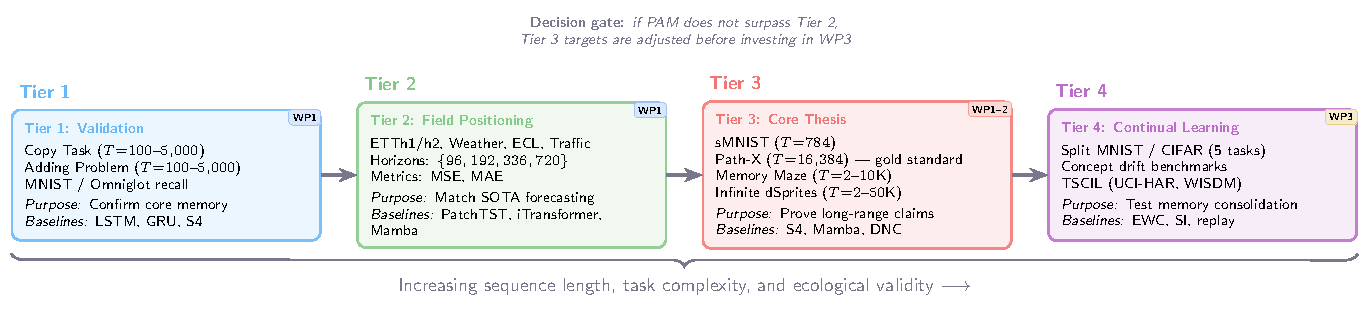
\includegraphics[width=\textwidth, clip]{figures/benchmark-tiers.pdf}
  \caption{\textbf{Four-tier benchmark hierarchy for PAM evaluation.} Increasing sequence length, task complexity, and ecological validity from left to right. WP badges indicate which work package addresses each tier. A decision gate between Tiers~2 and 3 ensures incremental validation before committing to the most ambitious benchmarks.}\label{fig:tiers}
\end{figure}

\paragraph{T1.1: Temporal Benchmarks and Architecture Scaling}
\textbf{Completed:} MNIST digit recall benchmark~\cite{gemici2017generative} (see Part I, Fig.~3).
\textbf{Planned:} Validate on Tier~1 (Copy Task, Adding Problem) and Tier~2 (ETT, Weather, ECL) benchmarks. Visual encoding via ResNet~\cite{he2016resnet}. Compare against GTMs~\cite{gemici2017generative}, VRNNs~\cite{chung2015vrnn}, LSTMs~\cite{hochreiter1997lstm}, S4~\cite{gu2021s4}, NTMs~\cite{graves2014ntm}, and DNCs~\cite{graves2016dnc}. Offline probing~\cite{park2023probing} will analyze learned representations.
\textit{Success criterion:} PAM must achieve ${\ge}90\%$ exact recall at $\sigma{=}0.3$ on Tier~1 tasks and MSE within 10\% of PatchTST on Tier~2.

\paragraph{T1.2: Inference Depth, Noise Robustness, and Capacity}
Systematically characterise the recall--noise--capacity landscape across $\sigma \in [0.0, 0.8]$ and $K \in [10, 500]$. Implement adaptive inference depth via prediction-error thresholding: at each iteration, compare the current prediction error against a learned threshold; terminate early when the error is below threshold, saving computation. Characterise interactions between slot count, HDC dimension, and forgetting rate under varying concept-drift speeds, providing design guidelines for WP2--3.
\textit{Success criterion:} Adaptive inference must achieve ${\geq}95\%$ of full-iteration accuracy at ${\leq}60\%$ of compute on the MNIST benchmark.

\paragraph{T1.3: Hierarchical Temporal Compression for Long-Horizon Memory}
Extend PAM with hierarchical time-scale factorisation: fast modules ($\Delta t{=}1$) process step-level inputs while slow modules compress episodes into semantic summaries via learned gating inspired by complementary learning systems~\cite{ramapuram2021kanerva}. The gating criterion---whether and when prediction error triggers consolidation from episodic to semantic memory---will be resolved experimentally using prediction-error statistics from T1.2. Evaluate on Tier~3 benchmarks: ``infinite dSprites'' ($T{=}2{,}000$--$50{,}000$) and Memory Maze ($T{=}2{,}000$--$10{,}000$)~\cite{pasukonis2022evaluating}. The key test is \textbf{Path-X} ($T{=}16{,}384$): only S4, Mamba, and a few others solve this benchmark; success here would demonstrate that HDC memory with iterative inference can match purpose-engineered SSMs on ultra-long-range tasks.

\subsubsection*{WP2: Causal Reasoning and Compositional Understanding \textnormal{(Lepperød, PD; Q2--Q4; Years 2--4)}}

WP2 extends PAM with active inference, causal world model learning, and subspace-based compositional reasoning. This WP integrates neurosymbolic components for explicit reasoning alongside statistical learning, while enabling the system to discover causal structure through interventions.

\paragraph{T2.1: Action-Augmented Temporal Predictive Coding}
Extend PAM to incorporate action nodes that modulate state transitions. Develop action-dependent prediction error computation across multiple timescales, including action-conditioned memory addressing, action-dependent update rules, and methods for maintaining temporal consistency. Design joint optimization of state predictions and action selections.
\textit{Success criterion:} Action-conditioned prediction error must correlate $r{>}0.7$ with observed state transitions in a controlled navigation task.

\paragraph{T2.2: Subspace Reasoning and Compositional Understanding}
Develop mechanisms for compositional, subspace-based reasoning within the PAM architecture. The core idea is to factorize latent spaces into semantically meaningful subspaces that can be \textit{composed algebraically} through HDC binding operations. Concretely, this means representing transformations as operations that compose exactly: a rotation followed by a colour change should produce the same result whether applied individually or as a single bound operation. Our preliminary PAMNCA results (24.7\% exact match on ARC with 1.47M parameters) validate this approach, and memory ablations show that distributed memory contributes 30--43\% of performance. Importantly, LoRA program decomposition experiments demonstrate that ARC programs are \textit{not} low-rank composable, motivating the shift to HDC algebraic composition which operates in $d{=}1000{+}$ dimensional space with guaranteed compositionality. We will implement: (i)~a lossless per-cell circular embedding for spatial structures; (ii)~algebraically exact primitives (rotation, reflection, translation, colour transformations) that compose via HDC binding; (iii)~a meta-learning pipeline (FOMAML~\cite{finn2017maml}) for few-shot program inference from support examples; and (iv)~HDC program storage enabling compositional search over the space of transformations. We evaluate compositional reasoning on abstract visual reasoning benchmarks including ARC~\cite{chollet2019arc}, letter-string analogies~\cite{mitchell1993analogy}, and bAbI multi-hop QA~\cite{weston2015babi}.
\textit{Success criterion:} Extend PAMNCA from 24.7\% to $>$40\% exact match on ARC through HDC algebraic composition. Compositional retrieval must generalise to out-of-distribution rules (e.g., novel rotation--colour combinations). Our preliminary miniARC search achieves 100\% OOD exact match on 4 novel rules. Figure~\ref{fig:comp} illustrates the approach.

\begin{figure}[ht]
  \centering
  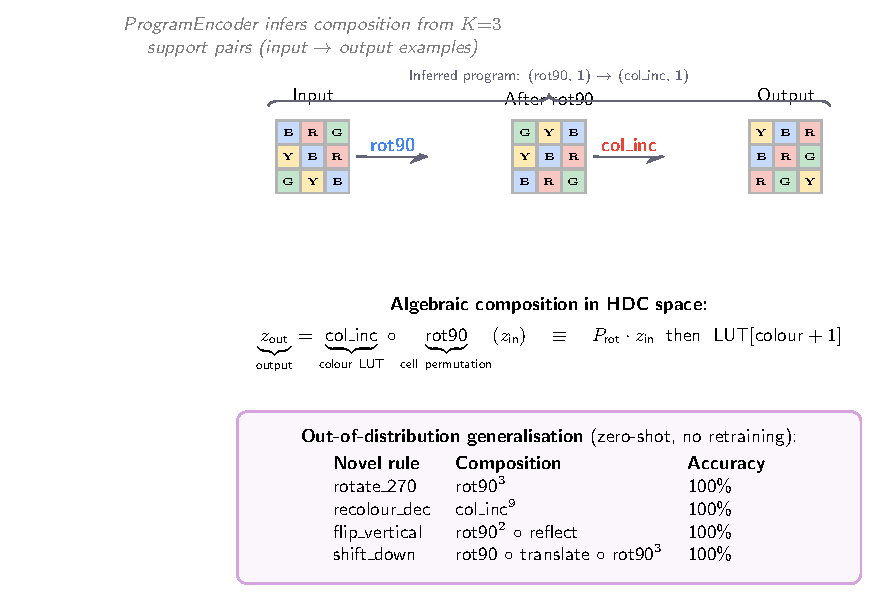
\includegraphics[width=0.85\textwidth, clip]{figures/compositional-reasoning.pdf}
  \caption{\textbf{Compositional reasoning through algebraic operations in HDC space.} A visual transformation (rotation + colour increment) is decomposed into composable primitives. The ProgramEncoder infers the composition from support examples. Algebraic composition guarantees out-of-distribution generalisation to novel rules without retraining (bottom table).}\label{fig:comp}
\end{figure}

\paragraph{T2.3: Causal World Model Learning through Active Inference}
Implement active inference for action selection balancing information gain and goal-oriented reward~\cite{friston2010free,rao2023active}. Develop causal discovery mechanisms through interventionist exploration: the agent executes targeted interventions (changing one variable while holding others fixed), observes the downstream effects, and updates its world model to encode directional causal relationships rather than mere correlations. This follows the ``interventionist'' approach to causal learning~\cite{scholkopf2021causal}: modules learn not just that ``opening a chest produces items'' but that ``the chest \textit{caused} items to appear,'' enabling counterfactual reasoning (``what if I hadn't opened the chest?''). Build on our work with NCA~\cite{kvalsund2024nca,kvalsund2026sensor} and proximal policy optimization~\cite{schulman2017ppo} for credit assignment.
\textit{Success criterion:} PAM with active-inference exploration must reach task completion $2{\times}$ faster than standard PPO on at least two benchmark environments.

\paragraph{T2.4: Orchestration Ablation and Evaluation}
Execute comprehensive ablation studies to quantify the contribution of each orchestration mechanism, distributed memory, and neurosymbolic component. Evaluate PAM on few-shot continuous control~\cite{mete2024few,yu2019meta} and long-horizon planning~\cite{pasukonis2022evaluating}. Investigate how PAM's computations map onto neural circuits by extending our established RNN framework~\cite{schoyen2023coherently,pettersen2024elife,pettersen2024nips} that demonstrates spontaneous development of grid, place, and border cells.
\textit{Success criterion:} PAM must achieve ${>}10$ percentage point improvement over LSTM baseline on Memory Maze ($T{>}500$ steps)---a deliberately intermediate gate; WP3 raises the bar to $T{=}10{,}000$ against stronger baselines (DQN, Dreamer). Orchestration ablations must show primary NCA/message-passing design outperforms at least two alternatives.

\subsubsection*{WP3: Long-Horizon Adaptation in Open-Ended Environments \textnormal{(Lepperød, PhD2; Q4--Q5; Years 3--5)}}

WP3 stress-tests PAM in environments demanding sophisticated planning, resource management, and adaptation to ever-changing dynamics. We adopt a tiered ambition structure:
\begin{itemize}[noitemsep,topsep=2pt]
  \item \textbf{Must achieve:} Memory Maze at $T{=}10{,}000$ with clear improvement ($>$10\,pp) over LSTM/DQN baselines.
  \item \textbf{Should achieve:} Simplified Minecraft tasks (navigation, basic crafting) via Python Malmo API~\cite{johnson2016malmo}.
  \item \textbf{Stretch goal:} Factorio production chains~\cite{kant2025factorio} requiring multi-step resource management across $T{>}10{,}000$ steps.
\end{itemize}

\paragraph{T3.1: Environment Development and Curriculum Design}
Design complex scenarios with varied challenges: resource management, crafting, building, combat, and exploration. Specific task designs include: (i)~Memory Maze~\cite{pasukonis2022evaluating} at increasing horizons ($T{=}2{,}000$--$10{,}000$); (ii)~multi-step crafting chains in Factorio where intermediate products must be stored and recalled across $T{>}10{,}000$ steps; (iii)~spatial exploration in Minecraft where the agent must build a mental map of a procedurally generated environment. Create a procedural generation pipeline varying task complexity, resource constraints, and causal dependencies. Implement adaptive curriculum using automatic curriculum learning~\cite{portelas2020acl} and intrinsic motivation~\cite{aubret2023intrinsic}: task difficulty increases only when the agent's competence (measured via prediction accuracy) exceeds a threshold. Observations via frozen ResNet~\cite{he2016resnet} encoder and game-state variables.

\paragraph{T3.2: Long-Horizon Active Inference Agent}
Integrate PAM into an interactive agent with a three-level policy hierarchy: (L1)~step-level motor primitives via PPO~\cite{schulman2017ppo}---low-level actions like movement, item use, crafting; (L2)~sub-goal selection via hindsight experience replay~\cite{andrychowicz2017her}---mid-level objectives like ``go to location X,'' ``collect item Y''; (L3)~strategic planning as symbolic goal vectors in HDC space~\cite{kanerva2009hyperdimensional,rajendran2024causal}---high-level plans like ``build a shelter before nightfall'' composed from bound sub-goal vectors. Each level maps to PAM modules operating at different temporal scales: L1 uses fast modules ($\Delta t{=}1$), L2 uses medium modules ($\Delta t{=}10$--$100$), and L3 uses slow modules ($\Delta t{=}100$--$1{,}000$) with persistent memory. Co-train through RL and self-supervised prediction objectives.

\paragraph{T3.3: Causal and Adaptive Learning Analysis}
Assess causal learning through interventions (changing game rules, introducing disturbances), counterfactual reasoning (simulating alternative scenarios), and analyzing the agent's ability to predict effects of its actions. Measure module specialization by analyzing activity patterns, stored information types, and task-specific contributions. Compare against DQN~\cite{mnih2015dqn}, PPO, RND~\cite{burda2018rnd}, Dreamer~\cite{hafner2018dreamer}, DINO-WM~\cite{zhou2024dinowm}, and MuZero~\cite{schrittwieser2019muzero}.
\textit{Success criteria:} (i)~PAM achieves $>$10\,pp improvement over DQN on Memory Maze at $T{>}5{,}000$ steps. (ii)~On Minecraft sub-tasks, PAM reaches task completion at least $1.5{\times}$ faster than PPO baseline. (iii)~Intervention experiments demonstrate $>$20\% accuracy in predicting novel action effects.

\subsection{Work and time schedule}

\begin{figure}[h!]
    \centering
    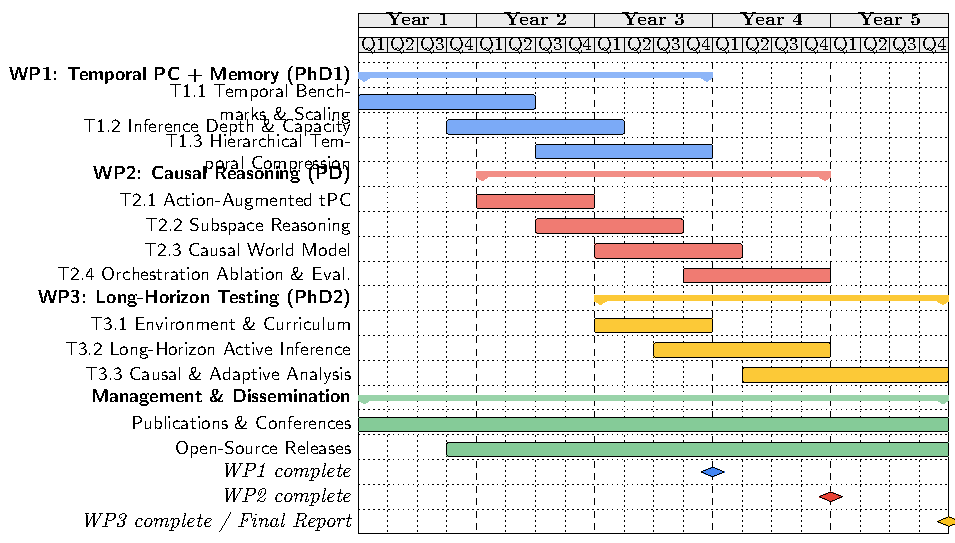
\includegraphics[width=\textwidth, clip]{figures/gantt-find.pdf}
    \caption{\textbf{FIND project Gantt chart (60 months).} WP1 (blue) Years 1--3, led by PhD1; WP2 (red) Years 2--4, led by PD; WP3 (yellow) Years 3--5, led by PhD2. Lepperød (PI, 50\%) provides scientific leadership across all WPs.}\label{fig:gantt}
\end{figure}


\noindent\textbf{Milestones:}
\begin{itemize}[noitemsep,topsep=2pt]
  \item \textbf{M1} (Month~12): PAM Tier~2 benchmarks complete; CORe50-NI results published.
  \item \textbf{M2} (Month~18): WP2 compositional reasoning prototype; extend PAMNCA with HDC composition.
  \item \textbf{M3} (Month~30): Memory Maze results at $T{=}10{,}000$.
  \item \textbf{M4} (Month~48): WP3 environment integration and agent evaluation.
  \item \textbf{M5} (Month~60): Final evaluation, open-source release, and benchmark suite.
\end{itemize}

\noindent\textbf{Estimated compute:} WP1: $\sim$20K GPU-hours; WP2: $\sim$30K GPU-hours (informed by PAMNCA's 15K hours for preliminary work); WP3: $\sim$50K GPU-hours. Total: $\sim$100K GPU-hours, covered by Simula eX3 and Sigma2 allocations.

\noindent\textbf{Team allocation:} Lepperød (PI, 50\%) provides scientific leadership across all WPs and leads WP2. The Postdoc (PD, 100\%) joins in Year~1 and co-leads WP2 with Lepperød, contributing to T2.1--T2.4. PhD1 (100\%) starts Year~1 and leads WP1 (T1.1--T1.3). PhD2 (100\%) starts Year~2 and leads WP3 (T3.1--T3.3). An additional PhD student may be hired in Year~3 depending on progress.

\subsection{Feasibility, risks, and contingency plans}

{\small
\noindent
\begin{tabularx}{\textwidth}{@{}p{1.3cm}Xp{0.8cm}p{0.8cm}X@{}}
\toprule
\textbf{Cat.} & \textbf{Description} & \textbf{Like.} & \textbf{Sev.} & \textbf{Mitigation} \\
\midrule
Scientific & Modular architecture fails to specialize. & Med & High & Progressive training with soft inductive biases; Gumbel-softmax entropy floor prevents module collapse. \\
 & Memory does not overcome catastrophic forgetting. & Med & High & Hybrid fast/slow memory with Bayesian consolidation; WTA write prevents slot mean-convergence. \\
 & tPC-KM fails to scale beyond MNIST. & Med & Med & Start with simplified environments; 4-tier benchmark hierarchy ensures incremental validation. \\
 & Compositional reasoning does not generalise beyond seen primitives. & Med & Med & Algebraic composition guarantees correctness by construction; FOMAML meta-learning for novel combinations. \\
Technical & Computational resources exceed expectations. & Med & Med & Sigma2 allocation + Simula eX3 cluster (${\sim}10^5$ GPU-hours); model distillation for efficiency. \\
 & Orchestration bottlenecks in information flow. & Med & High & Structured ablation ladder provides 4 fallback mechanisms ordered by complexity. \\
 & Active inference exploration is sample-inefficient. & Med & Med & Combine with imitation learning and adaptive curriculum; intrinsic motivation for efficient exploration. \\
Impl. & Environment integration (Minecraft/Factorio). & Med & Med & Simplified environment wrappers with fallback to Memory Maze; established Python APIs available. \\
Project & Recruitment of specialized expertise. & Med & Med & Leverage NORA network, ELLIS community, and international collaborations for candidate identification. \\
\bottomrule
\end{tabularx}
}

\noindent\textbf{Feasibility:} The preliminary results (98.1\% recall, $3.75{\times}$ less forgetting) demonstrate that the core architecture works. Each WP has independent value: even if WP3's most ambitious targets are not fully reached, WP1--2 produce publishable architectures and benchmarks. The structured ablation ladder in WP2 ensures that at least one orchestration mechanism will succeed. The 4-tier benchmark hierarchy provides natural checkpoints: if PAM does not surpass Tier~2, the Tier~3 targets are adjusted before investing in WP3 environments.

\subsection{Collaborations}

\noindent\textbf{Prof.\ Konrad Kording} (University of Pennsylvania): Bayesian decision theory and causal inference (WP2). One co-authored publication, ongoing collaboration since 2018. \textit{Tangible contribution:} Co-supervision of PD on causal world model formalism (T2.3); one PhD will visit Penn for 3 months in Year~3.

\noindent\textbf{Prof.\ Marc de Kamps} (University of Leeds): Computational neuroscience and compositional learning (WP2--3). Two co-authored publications, collaboration since 2016. \textit{Tangible contribution:} Collaboration on mean-field analysis of modular dynamics; joint workshops on biological plausibility of orchestration.

\noindent\textbf{Assoc.\ Prof.\ Blake Richards} (Mila/McGill): Normative models of hippocampal activity. Co-PI, PhD exchange program, ongoing since 2023. \textit{Tangible contribution:} PhD1 spends 6 months at Mila (Year~2) working on hippocampal models for WP1's hierarchical memory; joint publications on normative models of memory consolidation.

\noindent\textbf{Assoc.\ Prof.\ Arvind Kumar} (KTH): Neuromodulators in AI. Co-PI and co-author, ongoing since 2020. \textit{Tangible contribution:} Neuromodulatory gating mechanisms for memory consolidation (T1.3); joint supervision of PhD2.

\noindent\textbf{Prof.\ Stefan Leutgeb} (UC San Diego): Experimental spatial navigation. Visiting researcher 2017/2018, co-authored work submitted. \textit{Tangible contribution:} Experimental validation of PAM's spatial memory predictions against rodent place cell recordings.

\subsection{Integration into host institution}

Simula Research Laboratory is a Norwegian research institution with a strong track record in computational science. FIND will be hosted in the Department of Numerical Analysis and Scientific Computing (SCAN), within the BioAI group led by Lepperød. Simula provides:
\begin{itemize}[noitemsep,topsep=2pt]
  \item \textbf{Compute infrastructure:} Access to Simula's eX3 HPC cluster (A100/H100 GPUs) and national Sigma2 (Saga, Olivia) resources. WP3 RL experiments are estimated to require ${\sim}10^5$ GPU-hours (based on ${\sim}800$ GPU-hours per DreamerV3-scale training run $\times$ ${\sim}100$ experiments across curriculum stages and ablations). This exceeds Simula's internal allocation and motivates the additional equipment funding request.
  \item \textbf{Research environment:} Active AI research community, including the SURE-AI centre for industry collaboration, and connections to University of Oslo through Lepperød's adjunct professorship.
  \item \textbf{Training programs:} Simula Academy for researcher development; NORA Research School for PhD training; established supervision track record (2 PhDs completed, 4 in progress).
\end{itemize}

\subsection{Recruitment and ethics}

\noindent\textbf{Recruitment:} PhD and postdoc positions will be advertised internationally through NORA, ELLIS, and Simula's networks. We actively seek diverse candidates and will leverage our international collaborations for candidate identification. Simula's competitive salaries and Oslo's quality of life support strong recruitment.

\noindent\textbf{Ethics:} This research focuses on fundamental methods development in controlled game environments. No human subjects, animal data, or personal data are involved. We will follow Simula's Code of Ethics, the EU Ethics Guidelines for Trustworthy AI, and the EU AI Act. Beyond the project, applications of FIND technology would require evaluation of biases, security, and data governance.

\subsection*{Funding ID}

\begin{tabular}{p{3cm}p{3cm}p{6cm}p{2cm}}
\toprule
\textbf{Funder} & \textbf{Amount} & \textbf{Subject} & \textbf{Status} \\
\midrule
Simula internal & 4.5 MNOK/yr & BioAI group baseline funding & Active \\
RCN IKTPLUSS & 12 MNOK & PASSION: AI safety and alignment & Submitted \\
RCN FRIPRO & 10 MNOK & FIND (FRIPRO version): NeuroAI memory & Not funded \\
RCN IKTPLUSS & 12 MNOK & constrAIn: Constrained AI methods & Submitted \\
\bottomrule
\end{tabular}

\noindent The proposed ERC project is distinct from all listed funding. The FRIPRO FIND application (3-year, smaller scope) was not funded; the ERC proposal represents a substantially expanded 5-year programme with WP2 (compositional reasoning, validated by PAMNCA on ARC), WP3 (open-ended environments), the postdoc position, and substantial preliminary results (CORe50 continual learning, ARC program synthesis, HDC compositional reasoning benchmarks) not available at the FRIPRO submission.

\printbibliography[title={References}]
